 % The main file for CAMP reports
 % Don't put any content in here. 
 % Don't even include content files by using \input or \inlcude. 
 % Put your content to TEXT.TEX or include it there using \input.
 % Uses:
 %		SETTINGS.TEX	contains the settings for this document
 %		COMMANDS.TEX	contains commands which can be used while writing
 %		INFO.TEX			contains the author, title and so on for the cover
 %		COVER.TEX			formats the front cover of the document
 %		ABSTRACT.TEX	contains the abstract to be included (if needed)
 %		TEXT.TEX			contains the actual content of the document
 %		BIB.BIB				containt the BibTeX entries for the document
 
 
%% Draft document mode
%% Final document
\documentclass[11pt,a4paper,bibtotoc,idxtotoc,headsepline,footsepline,footexclude,BCOR12mm,DIV13]{scrbook}

%\documentclass[11pt,a4paper,bibtotoc,idxtotoc,headsepline,footsepline,footexclude,BCOR20mm,DIV10]{scrbook}

% KOMA-Optionen:
%  bibtotoc: include bibliography in table of contents
%  idxtotoc: include index in table of contents
%  headsepline: use horizontalline under heading
%  BCOR: binding correcion (Bindungskorrektur) (e.g.: BCOR5mm)
%  DIV: Number of sheet sections (used for layout) (e.g.: DIV12) 



% include title and author information for the cover
% Set here the title, authors and other stuff to be used for the cover
% This file is used by MAIN.TEX

% set title, authors and stuff for the cover
\def\doctype{Bachelorarbeit in Informatik}
\def\title{Cydonia 43: a nonviolent tactical multiplayer shooter}
\def\titleGer{Cydonia 43: Ein gewaltfreier Multiplayer-Taktik-Shooter}
\def\author{Florian Kick}
\def\date{15. September 2013}
\def\supervisor{Prof. Bernd Br{\"u}gge, Ph.D.}
\def\advisor{Dr. Damir Ismailovi{\'c}}

% text to appear in the footer
\def\footertext{}

% include settings
% Included by MAIN.TEX
% Defines the settings for the CAMP report document

%\renewcommand{\sectfont}{\normalfont \bfseries}        % Schriftart der Kopfzeile

% manipulate footer
%\usepackage{scrpage2}
%\pagestyle{scrheadings}
%\ifoot[\footertext]{\footertext} % \footertext set in INFO.TEX
%\setkomafont{pagehead}{\normalfont\rmfamily}
%\setkomafont{pagenumber}{\normalfont\rmfamily}

\usepackage{fancyhdr}

%% allow sophisticated control structures
\usepackage{ifthen}

% use Palatino as default font
\usepackage{palatino}

% enable special PostScript fonts
\usepackage{pifont}

% make thumbnails
\usepackage{thumbpdf}

%to use the subfigures
\usepackage{subfigure}


%\usepackage{colortbl}


%% show program code\ldots
%\usepackage{verbatim}
%\usepackage{program}

%% enable TUM symbols on title page
\usepackage{styles/tumlogo}


\usepackage{multirow}

%% use colors
\usepackage{color}

%% make fancy math
%\usepackage{amsmath}
%\usepackage{amsfonts}
%\usepackage{amssymb}
%\usepackage{textcomp}
%\usepackage{yhmath} % f�r die adots 
%% mark text as preliminary
%\usepackage[draft,german,scrtime]{prelim2e}

%% create an index
%\usepackage{makeidx}

% for the program environment
\usepackage{float}

%% load german babel package for german abstract
%\usepackage[german,american]{babel}
\usepackage[english,ngerman]{babel}
\selectlanguage{ngerman}

% use german characters as well
\usepackage[latin1]{inputenc}       % allow Latin1 characters

% use initals dropped caps - doesn't work with PDF
%\usepackage{dropping}


%\usepackage{styles/shortoverview}
%----------------------------------------------------
%      Graphics and Hyperlinks
%----------------------------------------------------

%% check for pdfTeX
\ifx\pdftexversion\undefined
 %% use PostScript graphics
 \usepackage[dvips]{graphicx}
 \DeclareGraphicsExtensions{.eps,.epsi}
 \graphicspath{{figures/}{figures/review}} 
 %% allow rotations
 \usepackage{rotating}
 %% mark pages as draft copies
 %\usepackage[english,all,light]{draftcopy}
 %% use hypertex version of hyperref
 \usepackage[hypertex,hyperindex=false,colorlinks=false]{hyperref}
\else %% reduce output size \pdfcompresslevel=9
 %% declare pdfinfo
 %\pdfinfo { 
 %  /Title (my title) 
 %  /Creator (pdfLaTeX) 
 %  /Author (my name) 
 %  /Subject (my subject	) 
 %  /Keywords (my keywords)
 %}
 %% use pdf or jpg graphics
 \usepackage[pdftex]{graphicx}
 \DeclareGraphicsExtensions{.jpg,.JPG,.png,.pdf,.eps}
 %\graphicspath{{figures/}} 
 
 %% allow rotations
 \usepackage{rotating}
 %% use pdftex version of hyperref
 \usepackage[pdftex,colorlinks=true,linkcolor=red,citecolor=red,%
 anchorcolor=red,urlcolor=red,bookmarks=true,%
 bookmarksopen=true,bookmarksopenlevel=0,plainpages=false%
 bookmarksnumbered=true,hyperindex=false,pdfstartview=%
 ]{hyperref}
%
%\usepackage[pdftex,colorlinks=false,linkcolor=red,citecolor=red,%
% anchorcolor=red,urlcolor=red,bookmarks=true,%
% bookmarksopen=true,bookmarksopenlevel=0,plainpages=false%
% bookmarksnumbered=true,hyperindex=false,pdfstartview=%
% ]{hyperref}
\fi




%% Fancy chapters
%\usepackage[Lenny]{fncychap}
%\usepackage[Glenn]{fncychap}
%\usepackage[Bjarne]{fncychap}

%\usepackage[avantgarde]{quotchap}

%\usepackage[style=numeric,backend=biber]{biblatex}
%\usepackage{natbib}
\usepackage[babel,german=quotes]{csquotes}
%\addbibresource{bibliography/literature.bib}

% set the bibliography style
%\bibliographystyle{styles/bauermaNum}
%\bibliographystyle{alpha}
\bibliographystyle{styles/myapalike}

% include commands
% Commands to be used within the TUM report document
% Included by MAIN.TEX
% Please include your own cool commands here. 
% Be only sure to comment it sufficiently so others can use it.

%-------------------------------------------------------------
%                      Own Commands
%-------------------------------------------------------------


%-------------------------------------------------------------
% math stuff -------------------------------------------------

% nice R, N, C
\newcommand{\nat}{\mathbb{N}}
\newcommand{\real}{\mathbb{R}}
\newcommand{\compl}{\mathbb{C}}



% norm
\newcommand{\norm}[1]{\left\| #1 \right\|}

% un demi
\newcommand{\half}{\frac{1}{2}}

% parantheses
\newcommand{\parenth}[1]{ \left( #1 \right) }
\newcommand{\bracket}[1]{ \left[ #1 \right] }
\newcommand{\accolade}[1]{ \left\{ #1 \right\} }
%\newcommand{\angle}[1]{ \left\langle  #1 \right\rangle }

% partial derivative: %#1 function, #2 which variable
% simple / single line version
\newcommand{\pardevS}[2]{ \delta_{#1} f(#2) }
% fraction version
\newcommand{\pardevF}[2]{ \frac{\partial #1}{\partial #2} }

% render vectors: 3 and 4 dimensional
\newcommand{\veciii}[3]{\left[ \begin{array}[h]{c} #1 \\ #2 \\ #3	\end{array} \right]}
\newcommand{\veciv}[4]{\left[ \begin{array}[h]{c} #1 \\ #2 \\ #3 \\ #4	\end{array} \right]}

% render matrices: 3  dimensional (arguments in row first order)
\newcommand{\matiii}[9]{\left[ \begin{array}[h]{ccc} #1 & #2 & #3 \\ #4 & #5 & #6 \\ #7 & #8 & #9	\end{array} \right]}
%DOESN'T WORK,DON'T KNOW WHY \newcommand{\mativ}[16]{\left[ \begin{array}[h]{cccc} #1 & #2 & #3 & #4 \\ #5 & #6 & #7 & #8 \\ #9 & #10 & #11 & #12 \\ #13 & #14 & #15 & #16 \end{array} \right]}


%-------------------------------------------------------------
%-------------------------------------------------------------


%-------------------------------------------------------------
% some abreviations ------------------------------------------
\newcommand{\Reg}{$^{\textregistered}$}
\newcommand{\reg}{$^{\textregistered}$ }
\newcommand{\Tm}{\texttrademark}
\newcommand{\tm}{\texttrademark~}
\newcommand {\bsl} {$\backslash$}

%-------------------------------------------------------------
%-------------------------------------------------------------


%-------------------------------------------------------------
% formating --------------------------------------------------

% Theorem & Co environments and counters
\newtheorem{theorem}{Theorem}[chapter]
\newtheorem{lemma}[theorem]{Lemma}
\newtheorem{corollary}[theorem]{Corollary}
\newtheorem{remark}[theorem]{Remark}
\newtheorem{definition}[theorem]{Definition}
\newtheorem{equat}[theorem]{Equation}
\newtheorem{example}[theorem]{Example}
\newtheorem{algorithm}[theorem]{Algorithm}

% inserting figures
\newcommand{\insertfigure}[4]{ % Filename, Caption, Label, Width percent of textwidth
	\begin{figure}[htbp]
		\begin{center}
			\includegraphics[width=#4\textwidth]{#1}
		\end{center}
		\vspace{-0.4cm}
		\caption{#2}
		\label{#3}
	\end{figure}
}




% referecing figures

\newcommand{\refFigure}[1]{ %label
	figure \ref{#1}
}
\newcommand{\refChapter}[1]{ %label
	chapter \ref{#1}
}

\newcommand{\refSection}[1]{ %label
	section \ref{#1}
}

\newcommand{\refParagraph}[1]{ %label
	paragraph \ref{#1}
}

\newcommand{\refEquation}[1]{ %label
	equation \ref{#1}
}

\newcommand{\refTable}[1]{ %label
	table \ref{#1}
}




\newcommand{\rigidTransform}[2]
{
	${}^{#2}\!\mathbf{H}_{#1}$
}

%code, in typewriter
\newcommand{\code}[1]
 {\texttt{#1}}

% comment that appears on the border - very practical !!!
\newcommand{\comment}[1]{\marginpar{\raggedright \noindent \footnotesize {\sl #1} }}

% page clearing
\newcommand{\clearemptydoublepage}{%
  \ifthenelse{\boolean{@twoside}}{\newpage{\pagestyle{empty}\cleardoublepage}}%
  {\clearpage}}


%-------------------------------------------------------------
%-------------------------------------------------------------


\newcommand{\etAl}{\emph{et al.}\mbox{ }}


%\makeindex
	%% inter line spacing
%\linespread{1.0}

\makeglossary

\begin{document}

	\frontmatter
	
	
	% The front cover for the TUM report document.
% Included by MAIN.TEX


%--------------------------------------------------
% The Front Cover
%--------------------------------------------------

% The front cover for the TUM document.
% Included by MAIN.TEX


%--------------------------------------------------
% The Front Cover
%--------------------------------------------------

% correct BCOR - undo at the end !!!
\def\bcorcor{0.15cm}
\addtolength{\hoffset}{\bcorcor}

\thispagestyle{empty}

 \vspace{4cm}
\begin{center}
	       \oTUM{4cm}
	   
	   \vspace{5mm}     
	   \huge FAKULT{\"A}T F{\"U}R INFORMATIK\\ 
	   \vspace{0.5cm}
	 \large DER TECHNISCHEN UNIVERSIT{\"A}T M{\"U}NCHEN\\
    \vspace{1mm}
        
	\end{center}
		

\vspace{15mm}
\begin{center}

   {\Large \doctype}

  \vspace{20mm}
  
  {\huge\bf \title}\\%[3ex]
  
  
  \vspace{15mm}
  
  
  {\LARGE  \author}
  
  \vspace{10mm}
  
  \begin{figure}[h!]
  \centering
   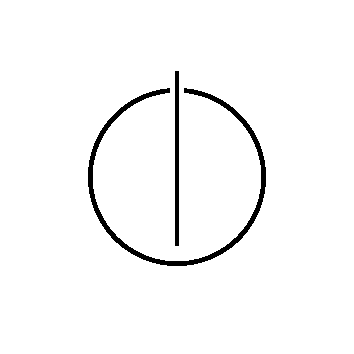
\includegraphics[width=4cm]{styles/informat.png}
  \end{figure}
  
  \end{center}
%	\clearemptydoublepage
%	
%	% The titlepage for the CAMP report document.
% Included by MAIN.TEX


%--------------------------------------------------
% The title page
%--------------------------------------------------

% correct BCOR - undo at the end !!!
\def\bcorcor{0.15cm}
\addtolength{\hoffset}{\bcorcor}

\thispagestyle{empty}

 \vspace{10mm}
\begin{center}
	       \oTUM{4cm}
	   
	   \vspace{5mm}     
	   \huge FAKULT{\"A}T F{\"U}R INFORMATIK\\ 
	   \vspace{0.5cm}
	 \large DER TECHNISCHEN UNIVERSIT{\"A}T M{\"U}NCHEN\\
        
	\end{center}
		

\vspace{10mm}
\begin{center}

   {\Large \doctype}

  \vspace{10mm}
  
  {\LARGE \title}\\
  
  
  \vspace{10mm}
  
  
  {\LARGE  \titleGer}\\
  
  
  \vspace{10mm}

    %\hfill
    \begin{tabular}{ll}
	   \Large Verfasser: & \Large \author \\[2mm]
	   \Large Aufgabensteller: & \Large \supervisor\\[2mm]				
	   \Large Betreuer: & \Large \advisor\\[2mm]
	   \Large Abgabedatum: & \Large \date
	 \end{tabular}
	 
	 \vspace{5mm}
	 
	 \begin{figure}[h!]
  \centering
   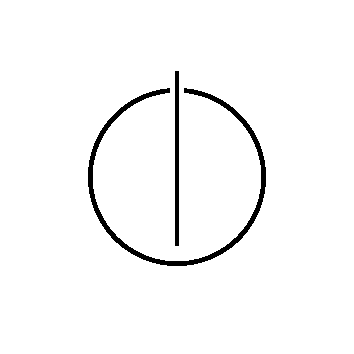
\includegraphics[width=4cm]{styles/informat.png}
  \end{figure}
   

\end{center}

% undo BCOR correction
\addtolength{\hoffset}{\bcorcor}
	
	
%	\input{components/cover_maschmeyer}
	\clearemptydoublepage
	
	% The titlepage for the CAMP report document.
% Included by MAIN.TEX


%--------------------------------------------------
% The title page
%--------------------------------------------------

% correct BCOR - undo at the end !!!
\def\bcorcor{0.15cm}
\addtolength{\hoffset}{\bcorcor}

\thispagestyle{empty}

 \vspace{10mm}
\begin{center}
	       \oTUM{4cm}
	   
	   \vspace{5mm}     
	   \huge FAKULT{\"A}T F{\"U}R INFORMATIK\\ 
	   \vspace{0.5cm}
	 \large DER TECHNISCHEN UNIVERSIT{\"A}T M{\"U}NCHEN\\
        
	\end{center}
		

\vspace{10mm}
\begin{center}

   {\Large \doctype}

  \vspace{10mm}
  
  {\LARGE \title}\\
  
  
  \vspace{10mm}
  
  
  {\LARGE  \titleGer}\\
  
  
  \vspace{10mm}

    %\hfill
    \begin{tabular}{ll}
	   \Large Verfasser: & \Large \author \\[2mm]
	   \Large Aufgabensteller: & \Large \supervisor\\[2mm]				
	   \Large Betreuer: & \Large \advisor\\[2mm]
	   \Large Abgabedatum: & \Large \date
	 \end{tabular}
	 
	 \vspace{5mm}
	 
	 \begin{figure}[h!]
  \centering
   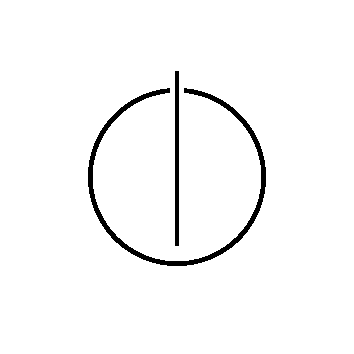
\includegraphics[width=4cm]{styles/informat.png}
  \end{figure}
   

\end{center}

% undo BCOR correction
\addtolength{\hoffset}{\bcorcor}
	
	
	\clearemptydoublepage


\thispagestyle{empty}
\selectlanguage{german}
	\vspace*{0.8\textheight}
	\noindent
	Ich versichere, dass ich diese Diplomarbeit selbst{\"a}ndig verfasst und nur 
	die angegebenen \\Quellen und Hilfsmittel verwendet habe.
	
	\vspace{15mm}
	\noindent
	M{\"u}nchen, den \today \hspace{5cm} \author
\selectlanguage{english}
\newpage
	
	\clearemptydoublepage
\phantomsection
\addcontentsline{toc}{chapter}{Acknowledgements}	


%\chapter*{Acknowledgements}

\vspace*{2cm}

\begin{center}
{\Large \bf Acknowledgments}
\end{center}

\vspace{1cm}




If someone contributed to the thesis... might be good to thank them here.
	
	% Abstract for the TUM report document
% Included by MAIN.TEX


\clearemptydoublepage
\phantomsection
\addcontentsline{toc}{chapter}{Abstract}	





\vspace*{2cm}
\begin{center}
{\Large \bf Abstract}
\end{center}
\vspace{1cm}

An abstracts abstracts the thesis!

	\tableofcontents
  
  %\clearemptydoublepage

\phantomsection
\addcontentsline{toc}{chapter}{Outline of the Thesis}

\begin{center}
	\huge{Outline of the Thesis}
\end{center}




%--------------------------------------------------------------------
\section*{Part I: Introduction and Theory}

\noindent {\scshape Chapter 1: Introduction}  \vspace{1mm}

\noindent  This chapter presents an overview of the thesis and it purpose. Furthermore, it will discuss the sense of life in a very general approach.  \\

\noindent {\scshape Chapter 2: Theory}  \vspace{1mm}

\noindent  No thesis without theory.   \\

%--------------------------------------------------------------------
\section*{Part II: The Real Work}

\noindent {\scshape Chapter 3: Overview}  \vspace{1mm}

\noindent  This chapter presents the requirements for the process.

	\mainmatter
	
	
		% Included by MAIN.TEX
% Put your content in here or include it by using \input (\include won't work)

\addtolength{\evensidemargin}{-12mm}

% ---------------------------------------------------------------------------
%
%Introduction and Background Theory
%
% ---------------------------------------------------------------------------
\part[Introduction and Background Theory]{Introduction and Background Theory}
\label{part:introAndBackgroundTheory}
\chapter{Einf�hrung}
\label{chapter:Introduction}

Seit langem herrscht in Politik und Gesellschaft Uneinigkeit �ber die Auswirkungen von Gewaltdarstellungen in
Computerspielen. Trotzdem sind solche stets in einigen Spielen enthalten gewesen. Besonders das Genre der Shooter ist f�r
seine detaillierten und intensiven Gewaltdarstellungen bekannt, der Anteil an Spielen mit hohen Altersbeschr�nkungen ist
darin besonders hoch (siehe Abb. \ref{figure:stigmafreigaben}). Dennoch definiert sich dieses Genre - entgegen der oft kritischen
�ffentlichen Meinung - nicht, oder zumindest nicht ausschlie�lich �ber die enthaltenen Gewaltdarstellungen.\\

\begin{figure}[htbp]
\centering
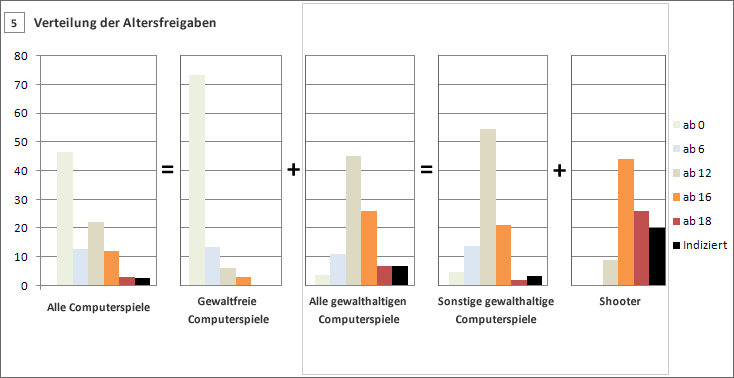
\includegraphics[width=0.8\textwidth]{images/stigmafreigaben}
\caption[Statistik der USK-Altersfreigaben nach Genres seit 1994]{Statistik der USK-Altersfreigaben nach Genres seit 1994\footnotemark}
\label{figure:stigmafreigaben}
\end{figure}
\footnotetext{Quelle: http://stigma-videospiele.de/wordpress/rechtslage/statistiken/}

\section{Zielsetzung}
Ziel dieser Arbeit ist die Analyse des Genres Multiplayer-Taktik-Shooter und die Erarbeitung eines Konzepts f�r einen
gewaltfreien Genrevertreter. Es soll gezeigt werden, dass das Spielprinzip des Shooters auch ohne Gewaltdarstellungen,
speziell ohne Schie�en auf und T�ten von Gegnern, funktioniert. Dazu sollen zum Einen die Eigenschaften, in denen sich
der Shooter au�er dem Schie�en noch von anderen Genres unterscheidet und damit selbst definiert, identifiziert und
verwendet werden. Zum Anderen sollen M�glichkeiten f�r neue Spielelemente gefunden und untersucht werden, die eine
eventuell entstehende L�cke im Konzept durch den Wegfall des Elements "`Schie�en"' f�llen oder ausgleichen k�nnen.\\

Es soll also eine M�glichkeit aufgezeigt werden, ein gutes Spiel zu entwickeln, das alle Eigenschaften und Elemente des
Shooters hat, die mit dem gewaltfreien Grundsatz vereinbar sind und somit das gleiche Klientel zufriedenstellt.

\begin{center}
Shooter - Schie�en + X $\rightarrow$ Spielqualit�t
\end{center}

Dabei ist mit Spielqualit�t Spielspa�, Motivation und Schwierigkeit gemeint, die an den Erwartungen von Shooterspielern
gemessen werden. Der Platzhalter X steht f�r Spielemente, die neu hinzugef�gt werden. Solche sollen in dieser Arbeit
gefunden und erprobt werden.

\chapter{Theorie und Hintergrund}
\label{chapter:BackgroundAndTheory}



Seit langem herrscht in Politik und Gesellschaft Uneinigkeit �ber die Auswirkungen von Gewaltdarstellungen in
Computerspielen. Trozdem sind solche stets in einigen Spielen enthalten gewesen. Besonders das Genre der Shooter ist f�r
seine detaillierten und intensiven Gewaltdarstellungen bekannt, der Anteil an Spielen mit hohen Altersbeschr�nkungen ist
darin besonders hoch\cite{stigmastatistik}. Dennoch definiert sich dieses Genre - entgegen der oft kritischen
�ffentlichen Meinung - nicht, oder zumindest nicht ausschlie�lich �ber die enthaltenen Gewaltdarstellungen. 

\section{Ziel}
Ziel dieser Arbeit war die Analyse des Genres Multiplayer-Taktik-Shooter und die Erarbeitung eines Prototypen-Konzepts f�r einen gewaltfreien Genrevertreter.\\

Ein Spiel nur mit dem Begriff "Shooter" zu beschreiben, und dann �ber das nicht vorhandensein von Gewaltdarstellungen zu
sprechen, klingt absurd und widerspr�chlich. Es verr�t schlie�lich schon der Name das wesentliche Spielelement, das
Schie�en, das sich kaum ohne Gewalt darstellen l�sst. M�glich w�re es, die Darstellung derart zu abstrahieren bzw. zu
verfremden, dass sie nicht mehr auf den ersten Blick als Abbildung von Gewalt erkennbar ist. Viele Spiele werden bewusst
in einem comic-�hnlichen Stil, oder im Fantasy- oder Sience-Fiction-Setting designed, um die �bertragbarkeit der
dargestellten Gewalt auf die Realit�t gering zu halten. Es geht hier jedoch nicht darum, ein Schie�spiel ohne Gewalt zu
entwickeln, sondern darum, die Eigenschaften, in denen sich der Shooter au�er dem Schie�en noch von anderen Genres
unterscheidet und damit selbst definieren l�sst, zu identifizieren und die weiteren Rahmenbedingen und
Alleinstellungsmerkmale des Shooters zu identifizieren, Je weiter man jedoch das Genre auf bestimmte Shooter eingrenzt,
desto mehr r�ckt das Schie�en in den Hintergrund. W�hrend man durch das erweitern der Spielbeschreibung

Spiele, die Gewalt (meist in Form von Kampfhandlungen) enthalten, gibt es gleicherma�en in den USK-Alterseinteilungen
"ab 12", "ab 16", "keine Jugendfreigabe" sowie bei Spielen, f�r die die USK die Kennzeichnung verweigerte (Siegel "keine Kennzeichnung"). Den Unterschied zwischen den ersten drei Stufen
macht vor allem der Realit�tsgrad, die �bertragbarkeitauf die Realit�t und den Alltag, sowie der auf den Sieler
ausge�bte Druck, gewaltt�tige Handlungen zu vollziehen, aus. "Keine Kennzeichnung" bedeutet z.B.,

\begin{itemize} 
  \item dass Spielinhalte Gewalttaten in der Alltagswirklichkeit legitimieren und Parallelen zur Realit�t nahelegen;
  \item dass das Spiel nur erfolgreich beendet werden kann, wenn Spielfiguren eliminiert werden, die nicht als Gegner auftreten;
  \item dass drastisch inszenierte und grafisch detailliert aufbereitete Gewalttaten gegen menschlich oder menschen�hnlich gestaltete Spielfiguren die Spielhandlung pr�gen;
  \item dass Kriegsbegeisterung vermittelt und Gewaltfolgen explizit bagatellisiert werden.
\end{itemize}

Das bedeutet, dass Gewalt in Spielen nicht unbedingt jugendgef�hrdend sein muss

\section{Definition und Abgrenzung: Multiplayer-Taktik-Shooter}
Heutige Computerspiele werden h�ufig einem der folgenden Genres zugesprochen: Shooter, Strategie, Rollenspiele. Diese
Liste ist nat�rlich weder vollst�ndig, noch ist die Zuordnung stets eindeutig. Alle Genres haben diverse Subgenres, es
gibt Spiele, die Elemente aus mehreren Genres vereinen, sog. Hybride. Au�erdem kann in fast jedem Genre noch nach
Singleplayer, Multiplayer oder Massive-Multiplayer unterschieden werden.\\

Um f�r die vorliegende Arbeit Unklarheiten und Missverst�ndnisse so gut es get zu vermeiden, soll im folgenden das
Subgenre der Multiplayer-Taktik-Shooter definiert und zu anderen Genres abgegrenzt werden. Die Definition l�sst sich
leicht anhand der einzelnen Namensbestandteile erl�utern.

\subsubsection{Shooter}
Ein Shooter ist ein Spiel, bei dem der Spieler einen einzelnen Avatar in einer virtuellen Welt steuert. Die
Steuerung erfolgt klassisch �ber Maus und Tastatur, wobei die Maus zum Umsehen und Zielen, die Maustasten zum Feuern der
Waffe und die Tastatur zum Bewegen benutzt wird. Das Spielziel ist meist das T�ten des Gegners mit einer Waffe.
Existiert ein alternatives Spielziel, so ist das Ausschalten des Gegners n�tig oder zumindest zutr�glich f�r das
Erreichen desselben.\\

Eine weitere Unterscheidung l�sst sich anhand der Perspektive feststellen. Von den drei
M�glichkeiten first-person, third-person und top-down ist erstere die bei Shootern am h�ufigsten eingesetzte. Auch
in der vorliegenden Arbeit soll diese verwendet werden.

\subsubsection{Taktik}
W�hrend in einem reinen Ego-Shooter der Spielablauf ausschlie�lich darauf ausgerichtet ist, Gegner zu t�ten und dabei
kein besonderes taktisches Vorgehen verlangt ist, sind in einem Taktik-Shooter unter anderem Fahigkeiten wie geschickte
Positionierung, Timing, Kenntnis der Umgebung, Abstimmung im Team gefordert. Das Schie�en auf den Gegner und die dabei
geforderte Pr�zision sind somit nicht allein spielentscheidend.

\subsubsection{Multiplayer}
Als Multiplayer-Spiel bezeichnet man ein Computerspiel, das �ber Netzwerk oder Internet von mehreren Spielern gemeinsam
gespielt wird. Die Avatare der Spieler befinden sich in einer gemeinsamen virtuellen Welt. Diese Welt wird von der
Spielmechanik so synchronisiert, dass alle Spieler Ereignisse und Ver�nderungen darin in gleicher Weise wahrnehmen
k�nnen. Gegner und Teammitglieder werden teilweise oder ausschlie�lich von realen Mitspielern gesteuert, was trotz der
stetig voranschreitenden KI-Entwicklung auch heute noch ein dynamischeres und realistischeres Verhalten der virtuellen
Spielfiguren erzeugt als bei sog. "BOTs" (engl. kurz f�r "robot"), vom Computer simulierten Mitspielern. 

\subsection{Weitere Abgrenzung}
Das Spiel l�uft in Runden mit stets der gleichen Ausgangssituation ab. Auf eine Handlung im Sinne eines Drehbuchs (wie
bei Singleplayer-Spielen �blich) sowie auf eine fortgesetzte Entwicklung der Spielwelt sowie des Charakters/Avatars (wie
bei Singleplayer- und Rollenspielen �blich) wird weitestgehend verzichtet.\\

Die Spielerzahl liegt in einem �berschaubaren Bereich. �blicherweise zwischen 10 und 64 Spielern pro Instanz, aber auch
Spiele mit bis zu 128 oder gar noch mehr Spielern sind bereits zu finden. Dennoch deutlich ist der Unterschied zu sog.
MMORPGs, bei denen oft mehrere tausend Spieler in einer Instanz spielen.\\

Bekannte Multiplayer-Taktik-Shooter im Sinne dieser Definition sind z.B. Counterstrike, Battlefield und Call of Duty.
Nicht darunter fallen Singleplayer-Spiele wie Tomb Raider, Splinter-Cell oder Shooter, denen der Taktik-Anteil fehlt,
wie z.B. Doom oder Unreal Tournament.\\


%
%% ---------------------------------------------------------------------------
%%
%% Analyse und Design
%%
%%% ---------------------------------------------------------------------------
\part[Analyse und Design]{Analyse und Design}
\label{part:analysisAndDesign}
\chapter{Ersatz f�r Gewaltdarstellungen}
\label{chapter:ViolenceSubstitution}


Ein Ansatz, bei den klassischen Shootern, die als Vorlage f�r das neue Spiel dienen sollen, Gewaltfreiheit zu erzwingen,
indem s�mtliche Gewaltdarstellungen entfernt werden, erweist sich als problematisch. Ein in dieser Art gek�rztes Spiel
w�re inhaltslos und somit langweilig, verliert also letztlich seine Daseinsberechtigung. Um den Spielwert aufrecht zu
erhalten, m�ssen also die Gewaltdarstellungen ver�ndert oder durch andere Spielelemente ersetzt werden. In typischen
R�tselspielen, Simulationen oder Strategiespielen wird der Spieler meist auch ohne Gewaltdarstellungen
unterhalten. Warum das bei Ego-Shootern - besonders im Multiplayerbereich - so schwierig ist, wird im folgenden
Abschnitt untersucht.


\section{Perspektive}

 
\section{Identifikation der Spielelemente}
Um die Gewaltdarstellungen aus dem Spiel entfernen zu k�nnen, m�ssen zuerst alle betroffenen Spielelemente identifiziert
werden. Dies soll im folgenden anhand bekannter Genrevertreter geschehen.

Hauptbestandteil eines Shooters ist - wie der Name schon erkennen l�sst - das Schie�en. Dies wird dem Spieler
�blicherweise durch ein Arsenal unterschiedlicher Waffen erm�glicht. W�hrend zum Beispiel Counterstrike reale
Waffenmodelle wie die AK47 oder die DesertEagle nachbildet, kommen in UnrealTournament futuristische Waffen wie
Laserkanonen zum Einsatz. Beiden gemeinsam ist, dass der Spieler mit diesen Waffen seine virtuellen Gegner durch
Beschuss verletzen und letztendlich t�ten kann. Ein get�teter Gegner scheidet - meist vor�bergehend - aus dem Spiel aus,
der Sch�tze bekommt Punkte. Neben der detaillierten Abbildung von Waffe und unter Umst�nden auch Projektil wird auch der
Tod des Gegners animiert, teils sehr blutig.

Abstrakter gesehen ist das Schie�en eine direkte Einwirkung auf den Gegner. Wesentliche Merkmale sind das Zielen auf die
virtuelle Spielfigur, das Aktivieren durch Tastendruck, sowie die negative, sch�digende und den Gegner in seinem
Spielablauf behindernde Wirkung. Ein hohes K�nnen (sog. Skill) erleichtert bzw. erm�glicht dem Spieler also das
Erreichen seines Spielziels, w�hrend es gleichzeitig dem Gegner das Erreichen seines Spielziels erschwert bzw. unm�glich
macht.


\chapter{Technische Details}
\label{chapter:TechnicalDetails}






%% ---------------------------------------------------------------------------
%%
%% Results and Conclusion
%%
%% ---------------------------------------------------------------------------
\part[Results and Conclusion]{Results and Conclusion}
\label{part:resultsAndConclusion}
\chapter{Schluss}
\label{chapter:Conclusion}

\chapter{Testing}
\label{chapter:Testing}


\section{Anwendertests}

Mehrfach w�hrend der Entwicklung wurde das Spiel Testpersonen vorgesetzt. Diese sollten ohne weitere Vorbereitung spielen und ihre Erfahrungen dann mitteilen.
Dabei wurden viele wesentliche Probleme und Schwachstellen aber auch positive und erhaltenswerte Elemente identifiziert. Die wichtigsten davon sollen im folgenden erl�utert werden.

Der im Rahmen dieser Arbeit entwickelte Spiele-Prototyp hatte zu einem fr�hen Entwicklungszeitpunkt folgenden
Spielablauf: Die Spielwelt bestand aus Bauklotz-�hnlichen W�rfeln, die die Spieler beliebig umbauen konnten. Ziel war es
ausgehend von einem Startpunkt als erster einen Zielpunkt zu erreichen. Dazu mussten Treppen, Br�cken und andere
Konstruktionen gebaut werden. Im Test mit mehreren Spielern zeigte sich, dass die M�glichkeit, dem Gegner W�nde in den
Weg zu bauen oder dessen Konstruktionen wieder zu zerlegen, nicht ausreichte um die Spieler zu motivieren. Ein Spieler
�u�erte sich folgenderma�en: "Mir fehlt was, um den anderen abzuknallen." Ebenso bot sich den Spielern kaum Raum,
kooperativ vorzugehen, was sich an der Aussage eines anderen Spielers erkennen l�sst: "Nein, ich wusste nicht, dass wir
im gleichen Team sind".
\chapter{Ergebnisse}
\label{chapter:Results}
\section{Ausblick}

Ist der Versuch, Shooter-Spieler von einem gewaltfreien Spiel zu �berzeugen, gegl�ckt? Diese Frage ist wohl noch nicht
beantwortet. Der Prototyp ist noch nicht ausgereift genug, um es mit anderen Spielen auf dem Markt aufzunehmen. Auch
haben erst eine kleine Auswahl von Spielern die Gelegenheit gehabt, Cydonia zu testen. Doch die ersten Versuche zeigen,
dass es sich lohnt, den eingeschlagenen Weg weiter zu gehen. 

\subsection{Die n�chsten Schritte}
Damit das Konzept von Cydonia Erfolg haben kann, muss aus dem Prototyp ein fertiges Spiel werden. Viele Details wurden
bei der Entwicklung vernachl�ssigt, einfach weil es zu viel Zeit kostet, sich mit ihnen zu befassen. Der Fokus lag auf
der Untersuchung des gewaltfreien Konzepts und seiner Elemente. Passende Avatarmodelle, Equipment-Modelle, Animationen,
Men�s, indivualisierbare Steuerung, detaillierte Ansicht der verf�gbaren Server, In-Game-Chat, Ping-Anzeige um nur ein
paar der Dinge zu nennen, die noch nicht fertig oder garnicht vorhanden sind. Wie in Abschnitt
\ref{subsubsection:Netcode} bereits erw�hnt, ist der Netzcode nur grundlegend implementiert und m�sste starkt optimiert
werden, vor allem wenn Cydonia auch �ber das Internet gespielt werden soll.

 


% ---------------------------------------------------------------------------
%
% Appendix
%
% ---------------------------------------------------------------------------

\part*{Appendix}
\addcontentsline{toc}{part}{Appendix}

\appendix %---------------------------------------

\chapter{Detailed Descriptions}
\label{chapter:DetailedDescriptions}
Here come the details that are not supposed to be in the regular text.




	

  \clearemptydoublepage

\bibliography{bibliography/literature}
%\printbibliography
 
\end{document}

